% !TeX spellcheck = en_US
% !TeX encoding = UTF-8
% !TeX root = ../document.tex

\chapter{Model Unspecific Search}

\section{Motivation}
A collision at a center-of-momentum energy of \SI{13}{\TeV} can create a large amount of different particles. Solely by combinatorics, it follows that a lot of different final states are accessible.

Most dedicated searches tend to focus on one or a few final states that represent the signature of the theory under investigation. This leaves many final states not examined, either because they are not covered by any new physics model or because there is no analysis group currently working on a corresponding theory.

One of the goals of the model unspecific search is to gain knowledge from these additional final states. Additionally, the model unspecific search aims to obtain a global interpretation of the agreement between simulation and observed data across a broad range of final states.

\section{Previous Works}
The approach of a model unspecific search is not a new concept: In 1998, a note about an unspecific search has been written at the L3 experiment (\ac{LEP})\cite{Hebbeker:GlobalComparisonL3}, and in 2004, a similar approach has been applied to data of the D0-experiment at the Tevatron proton-antiproton collider at Fermilab\cite{Biallass:ModelIndependentSearch}.

At \ac{CMS}, the analysis has been developed and regularly applied to observed data since 2009\cite{Schmitz:ModelUnspecificSearch,Hof:ImplementationModelIndependent,Dietz-Laursonn:ModelUnspecificSearch,Olschewski:StudyAlternativeStatistical,Brodski:ModelUnspecificSearch,Pieta:MUSiCModelUnspecific,Papacz:ModelUnspecificSearch,Albert:ExtensionModelUnspecific,Roemer:ModelUnspecificSearch,CMS:CMS-PAS-EXO-14-016,Knutzen:softwarereinterpretationmodel,Durchardt:MUSiCModelUnspecific}. 
This thesis bases on the most recent implementation of the \ac{MUSiC} analysis, which has recently been applied to analyze the dataset of the 2015 \ac{LHC} run\cite{Roemer:ModelUnspecificSearch} containing events with a integrated luminosity of \SI{2.3}{\per\femto\barn}.

A similar approach is also being pursued by the \ac{ATLAS} collaboration, who published several analyses using a model unspecific search at the \ac{LHC} at $\sqrt{s} = \SI{7}{\TeV}$\cite{ATLAS:ATLAS-CONF-2012-107}, \SI{8}{\TeV}\cite{ATLAS:ATLAS-CONF-2014-006} and \SI{13}{\TeV}\cite{ATLAS:ATLAS-CONF-2017-001}.

\pagebreak

\section{Procedure}
In the following sections, the existing analysis will be outlined.

The analysis starts out with reconstructed events of observed as well as \ac{MC} simulated data which have been centrally preprocessed by the \ac{CMS} collaboration.

As first step, requirements on events and physics objects are applied, discarding unwanted events and extracting objects for the \ac{MUSiC} analysis (sections \ref{sec:event_selection} and \ref{sec:reconstruction}).

Afterwards, each event is sorted into so-called \emph{event classes}, sets of events that share the same final state (\fref{sec:event_classes}).
For each event class, a set of kinematic variables of each event is calculated and \emph{kinematic distributions} are aggregated (\fref{sec:kinematic_distributions}).

Subsequently, an automated search algorithm finds the largest deviation between data and simulation within each kinematic distribution of each event class (\fref{sec:deviations_search}). Afterwards, the significance of each deviation is corrected for the look-elsewhere-effect using pseudo-experiments from \ac{SM}-only simulations (\fref{sec:global_significance}). 

Finally, the observed deviations are aggregated and the distribution of deviations is compared to the expected distribution given the \ac{SM}-only hypothesis as a measure for the global agreement between simulation and data (\fref{sec:ptilde_distribution}).

\section{Transverse Momentum and Energy}
\label{sec:transverse_quantities}

As prerequisite for the following sections it is helpful to introduce the so-called transverse quantities \emph{transverse momentum} and \emph{transverse energy}. This section provides a motivation and definition for both.

Interaction cross sections are often dependent on the amount of momentum involved. In t-channel diagrams, the entire momentum transfer can be measured by calculating the combined invariant mass of decay products.
In order to achieve this goal, one must know all four components of the momentum of all created particles. If the final state contains neutrinos, which are not detectable by the detector, this is not achievable.

In other experiments like \ac{LEP}, one could use conservation of momentum and the known momentum of colliding particles to reconstruct the neutrino four-momentum and the momentum transfer. At the \ac{LHC} this is also impossible: The total proton momentum is distributed unevenly between the constituent quarks and gluons and thus the momentum involved in a collision is only known up to statistical probability.

The mitigation pursued at \ac{CMS} is to only regard kinematics in the transverse plane, orthogonally to the beam pipe. Projection of the kinematic (three-)momentum onto the transverse plane gives the transverse momentum \pTvec.

There are other properties of the transverse momentum that make it an interesting quantity: It can be straightforwardly measured from the tracks since the magnetic field lines are approximately parallel to the beam direction and the Lorentz force only acts in the transverse plane. Additionally, the transverse momentum is not only invariant to the actual distribution of momenta within the proton, but also to Lorentz boosts along the $z$-axis. 

Assuming $p_x$, $p_y$, $E$ and $m$ can be observed directly (e.g. via track curvature) or indirectly (e.g. via particle identification), we can define the transverse momentum and transverse energy as follows:
\begin{align*}
\pTvec &\defeq \left( p_x, p_y, 0 \right)^T  \\
\pT &\defeq \abs{\pTvec} \\
\vec{E}_\mathrm{T} &\defeq E \frac{\pTvec}{\abs{\vec{p}}} = \frac{\pTvec}{\sqrt{1-\left(m/E\right)^2}}
\end{align*}

Note that in the approximation of massless ($m \approx 0$) particles: $\vec{p}_T = \vec{E}_T$. % $ = \vec{M}_T$.


\section{Event Selection}
\label{sec:event_selection}

The following section will discuss how events are selected to be used for the \ac{MUSiC} analysis. 

Since this thesis aims to be a general evaluation of the \ac{MUSiC} approach, we will not go deep into detail about the algorithms used, nor the exact parameter values. For the sensitivity studies in \fref{chap:sensitivity_studies}, however, specific values have to be chosen. If not explicitly stated otherwise, values of the 2015 analysis run are used and can be found in \cite{Roemer:ModelUnspecificSearch}.

\subsection{Triggers}
\newcommand{\trigger}[1]{\texttt{\detokenize{#1}}}
In \fref{sec:triggering} the triggering system has been introduced, a dedicated system that decides whether observed events are recorded to disk. In the vocabulary of an analyst, the term "trigger" does not only refer to the system itself, but also to the set of rules that are applied. In practice, triggering hardware is configured to run multiple sets of rules in a so-called \emph{trigger menu}, in order to maximize the usage of readout bandwidth without overloading the available resources.
The triggering decision is also simulated on \ac{MC} generated events: Using the same information available to the triggering system and a trigger emulator, each event is assigned tags about which decision lead to it being stored. 

Because multiple trigger configurations are running at the same time, the same event might end up in two separate trigger streams. Such duplicate events are removed in the analysis.
An additional problem arises within the first few \si{\GeV} beyond the \pT threshold: In this so-called \emph{turn-on} region, disagreement between observed data and simulation has been found which is accounted to insufficiencies in the simulation. Because of this, an additional minimum \pT threshold close above the trigger threshold is applied.

\Fref{tab:triggers} provides a reference of triggers used in the analysis. In comparison to the 2015 analysis, the \pT threshold of the single electron trigger has been raised from \SI{105}{\GeV} to \SI{115}{\GeV}. This choice ensures consistency between the 2015 and 2016 analysis for the study of the discovery potential.

\begin{table}
    \centering
    \begin{tabular}{l l l}
    \toprule
    Stream Name & trigger $p_\text{T, min}$ & custom $p_\text{T, min}$ \\
    \midrule
    \trigger{HLT_Ele115_CaloIdVT_GsfTrkIdT} & \SI{115}{\GeV} & \SI{120}{\GeV} \\
    \trigger{HLT_DoubleEle33_CaloIdL_GsfTrkIdVL_MW} & \SI{33}{\GeV}, \SI{33}{\GeV} & \SI{50}{\GeV}, \SI{50}{\GeV} \\
    \trigger{HLT_Mu50} & \SI{50}{\GeV} & \SI{53}{\GeV} \\
    \trigger{HLT_Mu17_TrkIsoVVL_Mu8_TrkIsoVVL_DZ} & \multirow{2}{*}{\SI{17}{\GeV}, \SI{8}{\GeV}} & \multirow{2}{*}{\SI{35}{\GeV}, \SI{35}{\GeV}} \\
    \trigger{HLT_Mu17_TrkIsoVVL_TkMu8_TrkIsoVVL_DZ} & & \\    
    \bottomrule
    \end{tabular}
    \caption{Triggers used in the \ac{MUSiC} analysis. Listed are the \ac{HLT} names. The double $X$ triggers require two particles, where the second minimal threshold lies much lower than the first. Additional identification requirements are applied as indicated by the name\cite[appendix C]{Roemer:ModelUnspecificSearch}. Note that the single electron trigger \pT threshold is higher than for the 2015 run.}
    \label{tab:triggers}
\end{table}


% CaloIdVT = Calo ID very tight
% GsfTrkId = Gaussian Sum Filter Track ID
% vvl = very very loose
% _MW = medium window (EGM trigger meeting anfang 2016)
% DZ = impact parameter cut

\subsection{Event Filters}
Event filters are used to mask off events that contain observations of unwanted detector behavior rather than physics content from a collision.
Undesirable experimental effects include defective modules, anomalous electronics noise, saturation of subsystems by calibration lasers or particles scattered on residual gas in the beam pipe. They sometimes mimic real particles and events and thus cause the trigger to store the event. In the offline analysis, these events are recognizable by a large momentum imbalance of the reconstructed particles, resulting in large values for \MET. Using a set of rules (so-called \MET-filters) established at \ac{CMS}, these events are excluded from the analysis. The list of applied filters can be found in \cite[appendix B]{Roemer:ModelUnspecificSearch}.

\section{Reconstruction and Selection of Objects}
\label{sec:reconstruction}

Now that a set of events to analyze has been established, we will focus on reconstruction selection of the particles within an event for our analysis. 

In practice, the reconstruction is performed centrally by \ac{CMS} working groups. For each particle, several reconstructed candidates are stored, from which the analyst can select. 
Besides selecting only the particles relevant for the analysis, one often chooses a \emph{working point} for particle identification criteria. The possible options are "tight", "medium" and "loose". Tight criteria are more strict, limiting the rate of misclassified particles at the cost of discarding some legitimate particles. On the other hand, loose criteria allow for more events, reducing the statistical uncertainty, with a higher probability of misclassification. As the name indicates, "medium" aims to provide a compromise between the two extremes.

For certain final states, it has been found that the probability of events being misclassified differs between \ac{MC} simulation and observation. However, the scaling factor to correct this effect has not been determined in all final states regarded by \ac{MUSiC}. Thus, to evade deviations that are caused by different misclassification rates, our particle selection generally requires tight identification criteria, except for light jets, which are selected with loose criteria to ensure a complete event description.

The following paragraphs aim to give a short overview over the reconstruction methods and object selection criteria used in the analysis. 

\subsection{Particle Flow}
\ac{MUSiC} uses the so-called \acfi{PF} algorithm\cite{CMS:CMS-PAS-PFT-09-001}, which aims to combine measurements from separate detector subsystems into a consistent picture of all stable particles in the event. This is achieved by allowing the separate particle reconstruction algorithms to use shared definitions and communicate, avoiding duplicate interpretation of the same data.

The \ac{PF} algorithm can be divided into three steps: Fitting of tracks and clustering, linking of tracks and clusters, reconstruction of particles.

In the first step, clusters of tracker cells that observed a current spike during the event are linked between the layers using a Kalman-filter, yielding reconstructed tracks. The same algorithm is also applied to the tracks of muons in the muon chambers. In the same step, clusters are found within the energy deposits of the calorimeters using a greedy clustering algorithm.

In the second step, tracks and clusters from the first step are linked to each other. Tracks from the inner tracking system are extrapolated to find matching clusters in the calorimeters. 
%Special care is taken for the signature of secondary electrons emitted by bremsstrahlung within the \ac{ECAL}. 
Similarly, clusters observed in the \ac{ECAL} as well as the \ac{HCAL} are related. Finally, tracks are matched between the inner tracker and the muon system.

The final step builds the actual particle candidates from the available information.
First, muons are identified if the momentum of linked tracks is compatible. Tracks that have been successfully associated to a muon are then removed from the track collection. Electrons are next: The tracks are refit using a Gaussian-Sum Filter and matched to energy deposits in the \ac{ECAL}. Again, information that has been related to an electron is removed from the track and cluster collections. The remaining tracks are afterwards associated to charged hadrons. Finally, the remaining energy clusters in \ac{ECAL} and \ac{HCAL} give rise to reconstructed photons and neutral hadrons respectively.

\subsection{Jets}
\label{sec:jets}

Jets form during the hadronization of quarks and gluons from the final state. The goal of jet reconstruction is to obtain the mass, energy and momentum of the originating parton or gluon.

In the detector, jets are measured as tracks and clusters of stable particles. Starting with the \ac{PF} objects, in the first step, charged contributions from pile-up are removed. The undesired tracks are selected by displacement from the primary vertex and then removed from the set of candidate particles.
After the correction, a jet clustering algorithm arranges the remaining particles into clusters. Within the \ac{MUSiC} analysis, the anti-$k_t$ algorithm\cite{Cacciari:antiktjet} with the characteristic radius $R = \num{0.4}$ is deployed. It uses pairwise recombination to form cone-like clusters around the hardest particles.

As output, one obtains a set of clusters, each containing multiple \ac{PF} objects. The combined four-vector of all particles within each cluster is calculated and assigned to the jet.

Measurements have shown that the energy resolution of jets is worse in observed data than in the \ac{MC} simulation. As a mitigation, the transverse momenta of simulated jets are smeared with a \pT and $\eta$-dependent factor\cite{TWiki:JetResolution}.
After the jet energy correction, the jets used within the \ac{MUSiC} analysis are selected using established jet-id criteria at the tight working point\cite{TWiki:JetID}. It ensures high data quality and low misclassification rates by requiring a minimum \pT threshold of \SI{50}{\GeV} and poses certain additional requirements on the composition of the jet.
% min pT: \SI{50}{\GeV}.

\subsection{Muons}
Muons are reconstructed from tracks in the inner tracker and in the muon system. For low energetic muons ($\pT < \SI{200}{\GeV}$), the momentum resolution of the inner tracker is superior to the muon chambers. Therefore, the momentum information is extracted from the tracker measurement, while the muon chambers are only used for selecting the tracks used. At high momenta ($\pT \geq \SI{200}{\GeV}$), the resolution can be increased by adding curvature measurement from the muon chambers and is therefore reconstructed using a combined methods.

The algorithms used for identification also depend on the muon momentum. Low energetic muons are identified using a series of cut-based criteria with a tight working point. High energetic muons are identified by a dedicated high-\pT algorithm which attempts to combine information from multiple muon chambers to achieve the best resolution\cite{TWiki:MuonIdentification}.

Both identification criteria require the muon to be fully contained in the detectable range ($\abs{\eta} < \num{2.4}$). The second main goal of the identification is to ensure that the muon candidate originates from the hard interaction. Secondary muons from jets or from pile-up collisions are vetoed based on displacements from the primary vertex, isolation criteria and a \pT threshold.

After a muon has been successfully selected for the analysis, close-by low-energetic electrons, photons and jets are removed from the event description. This avoids double-counting of physics content and thus strives to restore a consistent event description.

\subsection{Electrons}
Electrons are recognized by their curved track in the tracker and energy deposit in the \ac{ECAL}. For the reconstruction of low energetic electrons (below \SI{100}{\GeV}), the momentum information from the tracker and the \ac{ECAL} are combined using the estimated uncertainty as a weight. At higher energies, using only the \ac{ECAL} measurement has been shown to improve performance, thus the tracker momentum information is discarded.

The selection of electrons for the analysis is also applied in a piecewise manner: In the low energy regime, the tight cut-based electron identification criteria are required, while for high energies, the \acfi{HEEP} requirements\cite{TWiki:HEEP} are imposed. 

Both criteria aim to differentiate between electrons from the hard interaction and electrons from jets or pile-up. Again, a maximum displacement from the primary vertex is required, as well as a minimal isolation and a minimum \pT value. Jets are also suppressed by vetoing energy contributions in the \ac{HCAL}.

In addition, converted electrons and photons are vetoed by settings tight quality requirements on the electron track.

\subsection{Photons}
Photons do not leave tracks in the inner tracker. Besides that, their experimental signature resembles the signature of electrons. 
Therefore, photons are selected and identified in a similar matter. The \ac{MUSiC} analysis uses the cut-based photon identification criteria\cite{TWiki:PhotonID} over the entire energy range. 

In order to veto photons emitted as bremsstrahlung, photons with more than one signal in the tracker are discarded.

\subsection{Missing Transverse Energy}
Missing transverse energy, denoted by \MET, is a physics object characterizing momentum imbalance in the detector. The projected three-momentum is calculated from objects' corrected transverse energies as follows:
\begin{equation}
    \METvec \defeq - \sum_i \vec{E}_{T,i}
\end{equation}
Causes for missing transverse energy generally fall into one of two categories: Incorrect measurements, such as noisy, dead or asymmetric modules, and non-detectable particles. Neutrinos, for example, only interact very weakly and are therefore invisible for the detector. If one or more neutrinos are produced during the interaction, we can only observe their combined four momentum in terms of missing transverse energy. The same applies to hypothetical new physics particles which do not interact with the detector, making \MET an interesting physics object to work with.

All corrections that change the \pT value of \ac{PF} candidates (e.g. jet energy corrections) are passed onto the \MET calculation to preserve a consistent event description. 
Using similar arguments as for the other particles, only \MET with $\pT \geq \SI{100}{\GeV}$ is identified as object within the analysis.

\subsection{Possible Extensions}
The existing analysis can be extended to identify more particle types by their decay products, called \emph{tagging}. Possible tagging choices are \Pqb-tagging, \Ptau-tagging or \PZ-tagging.
This thesis will investigate the increase of sensitivity using \Pqb-tagging, as discussed below.

\subsection{b-Tagging}
\label{sec:b_tagging}

The goal of \Pqb-tagging is to distinguish jets from \Pqb-quarks ("\Pqb-flavored jets") from those originating from light quarks. One way of achieving this goal is to exploit the long lifetime of \PB-mesons. These mesons are formed during the hadronization of \Pqb-quarks and possess a comparably long lifetime of $\tau \approx \SI{1.5e-12}{\second}$\cite{ParticleDataGroup:ReviewParticlePhysics}. This allows \PB-mesons to travel up to a few centimeters before decaying.
With \ac{CMS}' tracking resolution of up to \SI{20}{\micro\meter} in the transverse and \SI{30}{\micro\meter} in the longitudinal direction\cite{CMS:CMS-PAS-BTV-15-001}, displacement of such magnitude can be resolved efficiently and is therefore an appropriate discriminator.

To introduce \Pqb-tagging in the \ac{MUSiC} analysis, the \acfi{CSVv2} algorithm\cite{CMSCollaboration:Identificationbquark} is used in addition to the jet requirements described in \fref{sec:jets}. The algorithm combines information of displaced tracks with information about displaced vertices in a multivariate analysis. The discriminator output is then compared to a threshold defined by the working point.
For the sensitivity studies, the "tight" working point with a discriminator threshold of \num{0.935} is used. Studies of the 2015 data and simulation have found that with the tight working point, approximately \SI{50}{\percent} of jets originating from \Pqb-quarks are correctly identified as such, while less than \SI{0.5}{\percent} of the \Pqb-tagged jets do not actually originate from \Pqb decays\cite{CMS:CMS-AN-2016-036}.


\section{Event Classes}
\label{sec:event_classes}

An event class is a set of events sharing the same final state. The final state is indicated by the name of the event class: All events in the class named \eventclass{2\Pe + 1\Pmu}, for example, contain two electrons and one muon in the final state.

There are three types of event classes: \emph{exclusive}, \emph{inclusive} and \emph{jet inclusive}.

Events in the exclusive event classes contain exactly the indicated (and no additional) particles in their final state. Each event thus belongs to exactly one exclusive event class.

Inclusive event classes are denoted with the suffix "\eventclass{+ X}" in the name (for example \eventclass{2\Pe + 1\Pmu + X}). Their final state contains the explicitly stated particles plus any number (including zero) of additional ones.  Each event can be assigned any number of inclusive event classes. One advantage of this procedure is a larger number of events per class which lower the statistical uncertainty. However, the correct combination of statistical results across multiple inclusive event classes is not trivial.

Jet inclusive event classes are denoted with the suffix "\eventclass{+ Njets}" in the event class name (e.g. \eventclass{2 \Pe + 1\Pmu + Njets}). Events contained in a jet inclusive event class may contain any number of jets in addition to the explicitly stated objects. This increases the number of events per class, as effects like initial or final state radiation are ignored, leading to reduced statistical uncertainties.

In any case, the kinematic variables are only calculated from the objects explicitly stated in the class name, in our example two electrons and one muon.
Event classes are dynamically generated based on the classified event content. In the next sections, the total number of generated event classes will be denoted with \nclasses.

\section{Kinematic Variables and Distributions}
\label{sec:kinematic_distributions}

For each event, the \ac{MUSiC} classification calculates three scalar variables from the particles defining the event class: the sum of transverse momenta, the invariant mass and the missing transverse energy.

As discussed in \fref{sec:transverse_quantities}, the sum of transverse momenta is the most directly observable variable and is invariant to Lorentz-boosts in the $z$ direction.
In the analysis it is denoted by \sumpT and calculated from the scalar sum of the magnitudes of the transverse momenta of all particles under consideration:
\begin{equation}
    \sumpT \defeq \sum_i \abs{\vec{p}_{\mathrm{T}, i}} 
\end{equation}

The invariant mass is, as mentioned before, very sensitive to resonances in the t-channel. If the event class definition contains missing transverse energy passing the selection criteria, the invariant mass will not be computed, instead the transverse mass is used. The variables are denoted with \Minv and \MT respectively and defined as:
\begin{align}
    \Minv &\defeq \sqrt{\left(\sum_i E_i\right)^2 - \left(\sum_i \vec{p}_i\right)^2} \\
    \MT &\defeq \sqrt{\left(\sum_i E_{T,i}\right)^2 - \left(\sum_i \vec{p}_{T,i}\right)^2}     
\end{align}

The third kinematic variable is missing transverse energy. 
This variable is only calculated if the event class definition explicitly contains \METvec (above the threshold of \SI{100}{\GeV}) and describes the magnitude of the missing transverse momentum \METvec:
\begin{equation}
    \MET \defeq \abs{\METvec} 
\end{equation}

From each of the kinematic variables, \emph{kinematic distributions}, histograms of the corresponding calculated variable, are aggregated. The bin size of these histograms is not constant, but instead chosen to match the estimated detector resolution in the variable under investigation. However, the bins are guaranteed to be at least \SI{10}{\GeV} wide.

\section{Systematic Uncertainties}
When comparing observed data to simulation, \emph{systematic uncertainties} have to be considered. For various reasons, one will never be able to exactly predict how many events will pass the analysis. Possible causes include inaccuracies in the theoretical prediction, uncertainty on how a particle affects the detector and statistical uncertainty from performing a counting experiment on independent events. 
Therefore, we are only able to estimate the observable event yield up to a certain interval. In this analysis, we assume that most of the uncertainties that arise can be modeled with a normal distribution and thus denote them with a mean value and a \SI{68}{\percent} confidence interval within $\pm 1 \sigma$ around the mean. The uncertainties are propagated onto the event yield of each kinematic bin and used in the subsequent automated search as well as the generation of pseudo-experiments.

There are multiple quantities involved in the calculation of the predicted number of events $N$. Here, we will categorize these effects into three groups:
\begin{equation}
N = \underbrace{\sigma}_\text{theory} \cdot \underbrace{\mathcal{L}}_{\substack{\text{independent} \\ \text{measurements}}} \cdot \underbrace{A \cdot \epsilon}_{\substack{\text{experimental} \\ \text{response}}}  
\end{equation}
This categorization will be used in the following sections, where we will give an overview about the currently implemented systematic uncertainties. As with \fref{sec:reconstruction}, the concepts are only roughly motivated, more comprehensive information and actual parameter values can be found in \cite{Roemer:ModelUnspecificSearch}.

\subsubsection{Theoretical Uncertainties}
The dominating theoretical uncertainty stems from the perturbative calculation of the cross section. In quantum field theory, the interaction potential is expanded in discrete orders. The computation of higher order terms is analytically impossible and can often only be estimated up to an uncertainty. Therefore, the \emph{cross section uncertainty} is chosen depending on the highest calculated order for a given sample, and lies between \num{5} and \SI{50}{\percent} of the cross section.

The second considered theoretical uncertainty deals with the parton density function. Its task is to model the distribution of momentum between quarks and gluons in a proton. As the underlying effects in the theory of \ac{QCD} are not completely understood, combined results from various deep inelastic scattering experiments are used. The uncertainty of these results is propagated onto the predicted yield by varying between multiple available result sets.

\subsubsection{Independent Measurements}
The systematic uncertainty on the luminosity directly affects the expected number of events. 
At any time, the current instantaneous luminosity is estimated by the activity in the pixel tracker. The measurement is complemented by a calibration from periodical precise van-der-Meer scans.
This procedure is sufficiently accurate, as its uncertainty is estimated to be only \SI{2.7}{\percent}\cite{CMS:CMS-PAS-LUM-15-001}.

The number of pile-up interactions within an event can be estimated from the total proton-proton cross section, combined with the instantaneous luminosity. The uncertainty of these independent measurements is propagated onto the number of pile-up collisions using a reweighting method to study the effect on the expected yield.

\subsubsection{Event-Dependent Uncertainties}
As discussed before, the energy of a reconstructed particle is estimated from the measured data of various detector components. The uncertainty on this mapping is called \emph{energy scale uncertainty} and is considered for all particles: jets, electrons, muons, photons and \MET. It is determined by studying differences between simulation and observed data of well-known physical processes. The uncertainty is then propagated onto the event by shifting the object momenta by $\pm \sigma(\pT)$ and repeating the classification. Note that the objects whose \pT values have been shifted may subsequently pass certain selection criteria and thus contribute to different bins or even different event classes than the original event.

Similarly to the energy scale uncertainty, the simulated detector resolution is subject to uncertainty. This uncertainty is determined from independent observations, such as cosmic muons and \PZ-decays, and is also propagated by shifting object momenta. The energy resolution uncertainty is only significant for muons and jets, depends on $\eta$ and \pT and is \SI{3} to \SI{5}{\percent} of the objects' momentum.

In addition to uncertainties on the measured momenta, we also consider uncertainties on the identification of particles. Two effects have to be taken into account: Particles may not be recognized with the correct type (\emph{identification efficiency}) or contributions that do not originate from particles might be incorrectly classified as particles (\emph{misidentification rate}). Ideally, the probability of these effects occurring would be the same in simulation as in observed data, therefore there are several techniques that aim to correct the \ac{MC} expectation.

To reproduce the identification probability of data in simulation, the expected yield is multiplied by so-called scale factors. The uncertainties of these scale factors are propagated by shifting the scale factors and observing the effects on the event yield.

The treatment of incorrectly identified objects is more difficult: For each identified particle, there is a nonzero chance that it may not actually correspond to the reconstructed particle type. To account for differences of this behavior between observation and prediction, we study incorrectly classified objects in the simulation. If an event contains one or more incorrectly classified objects, an uncertainty of \num{1} event is assigned to the corresponding bin (for electrons, muons and photons)\cite{Roemer:ModelUnspecificSearch}. 
For \Pqb-tagged jets, the mismatch of the misclassification rate between data and prediction has been studied in 2016 data and found to be up to \SI{30}{\percent}\cite[Fig. 73]{CMS:CMS-AN-2017-018}, so \num{0.3} events of uncertainty are assigned for each misclassified event. 

The actual misclassification rates depend on the final state but are in the order of \SI{1}{\percent} for most event classes.

\subsubsection{Statistical Uncertainty}
The amount of simulated \ac{MC} events is limited, mostly by computational costs. When comparing the scaled number of events to observed data, one has to take into account statistical effects of the discrete event production. The scaled number of events is calculated by multiplying the generated number of events $N$ with a scalar $s$. The statistical uncertainty on the generated number of events is derived from the standard deviation of the Poisson distribution: 
\begin{align}
    n &= s \cdot N, \quad \sigma_{\text{stat}, N} = \sqrt{N} \\
    \Rightarrow \sigma_{\text{stat}, n} &= s \sqrt{N} \\
    \Rightarrow \text{relative uncertainty} &= \frac{\sigma_{\text{stat}, n}}{n} = \frac{s \sqrt{N}}{s N} = \frac{1}{\sqrt{N}}
\end{align}
One can see that an increase in the number of simulated events directly decreases the statistical uncertainty on the prediction.

\section{Search for Deviations}
\label{sec:deviations_search}

After each event has been classified, the kinematic distributions have been aggregated and the systematic uncertainties have been propagated onto the event yield follows the automated search for deviations. The search is performed on each distribution of each event class separately as follows:
First, multiple connected bins are combined to a \emph{region}, according to the rules in  sections \ref{sec:search_space} and \ref{sec:region_veto}. Then, a test statistic \TS for each region is calculated (\fref{sec:test_statistic}). Of all possible connected bin combinations, the region with the lowest value of \TS, called \TSmin, is selected. This region will be called \acfi{RoI}. If two or more regions with the same value of \TSmin are found, the smallest one is classified as \ac{RoI}.

Subsequently, a global \ptilde-value for the region is calculated. This \ptilde-value expresses the probability of finding a deviation with $\TS \leq \TSmin$ anywhere within the distribution purely by chance. Details on the procedure can be found in \fref{sec:global_significance}.

\subsection{Search Space}
\label{sec:search_space}

The search is performed on so-called regions. A region is a set of adjacent bins and is represented by the combined number of expected and observed events as well as a combined uncertainty.

As we do not expect new physics to appear resonantly in the \sumpT and \MET kinematic distributions, each region within these distributions must consist of at least \num{3} adjacent bins. Within the \Minv and \MT distribution, narrow resonant deviations are possible, thus the minimal number of bins in these distributions is set to \num{1}. In addition, we employ a veto on regions where the simulation is incomplete, which is described in the next section.

The combined number of events and the combined uncertainty for each region is calculated as
\begin{align}
     N_{\text{total},\text{exp}} &= \sum_i N_{i, \text{exp}} \\   
     N_{\text{total},\text{obs}} &= \sum_i N_{i, \text{obs}} \\
     \sigma_\text{total} &= \sqrt{\sum_i \sigma_i^2 + 2 \sum_{i,j} \rho_{i,j}\sigma_i\sigma_j}
\end{align}
where $\rho_{i,j}$ is the correlation coefficient for the uncertainty $\sigma$ between the bins $i$ and $j$.

Some uncertainties, such as the statistical uncertainty on the simulated number of events, are completely uncorrelated between the bins. The correlation coefficient thus is $\rho_{i,j} = 0$ and the total uncertainty is the quadratic sum of the bin uncertainties.

Other uncertainties are correlated between bins. An example for this is the uncertainty on the luminosity measurement, which affects all bins of all distributions the same way. We treat any uncertainty that is assumed to be correlated to some extend as fully correlated ($\rho_{i,j} = 1$) and calculate the combined uncertainty as linear sum. This method possibly overestimates the total uncertainty, in case the correlation coefficient is somewhere between 0 and 1, leading to a lower sensitivity.

\subsection{Region Veto}
\label{sec:region_veto}
Although the analysis aims to cover as much phase space as possible by combining large amounts of \ac{MC} events, there are regions where the \ac{MC} description is incomplete. 
Because the null-hypothesis (the \acl{SM}) is not correctly represented in some areas, we must not probe for new physics in these regions, i.e. any statistical inference from these regions would be invalid.

Therefore, several rules have been identified and implemented in order to skip calculation of \TS values for incorrectly modeled regions. These rules may only depend on the \ac{SM} values, not on the observed data per region. In addition, note that any region is usually embedded in a larger region with a higher confidence in simulation. 

Some of the rules do not only depend on the region itself, but also on a \emph{neighborhood}. The neighborhood is defined as combination of adjacent bins below and above the region boundaries, \num{4} in each direction. In the neighborhood, we define a set of \emph{dominant neighborhood processes} as the set of processes with the largest contributions, which in total make up more than \SI{95}{\percent} of the total yield in the neighborhood.

The following rules are tested, if any of them matches, the region is vetoed, no \TS value is calculated and thus not considered for \ac{RoI}.

%\todo{was heißen die prozente? Antwort: prozent der regions vetoed durch regel. ACHTUNG: manche regions würden durch mehrere tests fallen, also prio... oder weglassen}
\begin{itemize}
    \item No or negative total \ac{MC} yield: $\Nmc \leq \num{0}$. %($\approx \SIrange{5}{15}{\percent}$).
    \item Any process contributes more than \SI{2}{\percent} of the event yield in the negative direction. %($\approx \SI{3}{\percent}$).
    \item Any process which has been identified as dominant in the neighborhood has no or negative total \ac{MC} yield. %($< \SI{1}{\percent}$).
    \item Region has large total statistical uncertainty: $\frac{\sigma_\text{stat}}{\Nmc} > \SI{60}{\percent}$. %($\approx \SIrange{5}{10}{\percent}$).
\end{itemize}

Negative total \ac{MC} yield can arise from few events with negative weights. In order to account for possible double counting between leading order matrix element calculations and parton showering, which is for some samples performed by a different application, \ac{MC} generators may assign negative weights to a small number of events\cite{Frixione:MatchingNLOQCD}.
Therefore, especially in phase space areas with few simulated events, situations can occur where only negative event weights contribute to a region. 
In these regions the original assumption, having enough events for a regression to the mean, is not fulfilled, thus the \ac{SM} is not correctly represented and the regions must be vetoed.

\subsection{Test Statistic}
\label{sec:test_statistic}

For each region, a test statistic is calculated. Its goal is to express "extremity" of a deviation based on the number of expected events \Nmc and their uncertainty \sigmamc, and the number of observed (or pseudo-observed) events \Ndata.

The choice of such a measure is ambiguous: All test statistics have strengths and weaknesses and are more or less sensitive in various areas of their three-dimensional input domain.
For the \ac{MUSiC} analysis, especially for the subsequent calculation of \ptilde, it is desirable to use a test statistic based on a null-hypothesis for which we can reliably generate pseudo-experiments. 

Ideally, the test statistic would express a local $p$-value directly, in order to be comparable to other \ac{CMS} results. However, as shown in the following section, only the ordering of \TS values is relevant within the \ptilde calculation and thus any test statistic $\TS(p)$ that is monotonous in $p$ will suffice.

In the following, we want to motivate the test statistic as used in the analysis.

The first (reasonable) assumption in the derivation is that the probability of observing a certain number of events given an exactly known prediction \Ntrue follows a Poisson distribution:
\begin{equation}
    \Pr(\Ndata | \Ntrue) = \frac{{\Ntrue}^\Ndata}{\Ndata!} e^{-\Ntrue}
\end{equation}

In context of a $p$-value which expresses the probability of obtaining a deviation equally or more extreme than the observed one just by chance, we have to sum over all "more extreme" cases. In case of an excess ($\Ndata \geq \Ntrue$), this is 
\begin{equation}
    p(\Ndata | \Ntrue) = \sum_{n = \Ndata}^{\infty} \frac{{\Ntrue}^n}{n!} e^{-\Ntrue}
    \label{eq:p_value_excess}
\end{equation}
For a deficit, the sum is finite and corresponds to:
\begin{equation}
    p(\Ndata | \Ntrue) = \sum_{n = 0}^{\Ndata} \frac{{\Ntrue}^n}{n!} e^{-\Ntrue}
    \label{eq:p_value_deficit}
\end{equation}

In reality, \Ntrue can never been known with perfect precision. Instead, our knowledge can be expressed by a probability density $\rho(x | \Nmc, \sigmamc)$ which is then folded into the $p$ value:
\begin{equation}
    p(\Ndata | \Nmc, \sigmamc) = \int_{-\infty}^\infty p(\Ndata | x) \cdot \rho(x | \Nmc, \sigmamc) \, \dd x
\end{equation}
Here, one can imagine that $x$ takes the role of all possible \Ntrue values and $\rho$ assigns different weights to contributions from equations \ref{eq:p_value_excess} and \ref{eq:p_value_deficit}.

In the case of \ac{MUSiC}, we apply the smearing procedure after deciding whether a region contains an excess or a deficit, which allows us to move the piecewise definition out of the integral:
\begin{equation}
    p(\Ndata | \Nmc, \sigmamc) = \begin{cases} \displaystyle
        \int_{-\infty}^\infty \rho(x | \Nmc, \sigmamc) \mathmakebox[30pt][c]{\displaystyle \sum_{n = 0}^{\Ndata}} \frac{x^n}{n!} e^{-x} \dd x & \Ndata < \Nmc \\
        \displaystyle \int_{-\infty}^\infty \rho(x | \Nmc, \sigmamc) \mathmakebox[30pt][c]{\displaystyle \sum_{n = \Ndata}^{\infty}} \frac{x^n}{n!} e^{-x} \dd x & \Ndata \geq \Nmc
    \end{cases}
\end{equation}

This is turn also implies that we treat contributions of the integral where e.g. $\Nmc < \Ndata < x$, as if they belong to an excess and thus sum up from \Ndata to infinity. This conservative choice of procedure is not expected to have a high impact to the results because it is also corrected during the calculation of \ptilde.

The choice of the prior $\rho(x | \Nmc, \sigmamc)$ is also not unambiguous: For previous \ac{MUSiC} publications and the signal study in this thesis, a truncated Gaussian prior is used:

\begin{equation}
    \rho_N(x | \Nmc, \sigmamc) = C(\Nmc, \sigmamc) \cdot \Theta(x) \cdot \exp(\frac{\left(x-\Nmc\right)^2}{2 \sigmamc^2})
\end{equation}
Here, $C(\Nmc, \sigmamc)$ is a normalization constant to correct for the truncated ($x < 0$) part of the normal distribution and $\Theta(x)$ denotes the step-function.

However, it has been under discussion in earlier theses\cite{Schmitz:ModelUnspecificSearch} to use a log-normal prior instead:
\begin{equation}
    \rho_{LN}(x | \Nmc, \sigmamc) = \frac{1}{\sqrt{2\pi}\abs{x}\ln(1 + \frac{\sigmamc}{\Nmc})} \exp(-\frac{1}{2}\left(\frac{\ln(x/\Nmc)}{\ln(1 + \frac{\sigmamc}{\Nmc})}\right)^2)
\end{equation}

The log-normal prior represents the multiplicative nature of uncertainties and features a larger coverage range, but has disadvantages concerning the generation of pseudo-experiments. In \fref{sec:lognormal_pvalue}, the alternative of a log-normal prior will be discussed in further detail.


%back to definition: sum of probabilities of more extreme events
%
%start using Poissonian probability
%include Gaussian prior: either normal or log normal

%
%most of the systematic uncertainties scale number of events in a region rather than a constant shift. examples: lumi, xsec, PDF, ID efficiency, misID


\subsection{Corrected Significance}
\label{sec:global_significance}

So far, we have only considered an estimator for the local magnitude of a deviation. In order to quantify and compare it, it has to be put in context: As the number of regions $n$ grows, the probability of finding a deviation with a significance of $\alpha$ increases, roughly $p \sim 1 - (1 - \alpha)^n$. The analysis accounts for this so-called \emph{look-elsewhere effect} by calculating a corrected post-trial $p$-value called \ptilde.
It expresses the probability of finding a deviation equally large or larger than the observed one somewhere in the distribution, solely by chance.

The simplest way of correcting the local magnitude would be to apply an analytical correction factor to it. A suitable correction factor could be estimated using combinatorics if the possible values of the local $p$-value were uncorrelated. This method is also called \emph{Bonferroni correction}\cite{Abdi:BonferroniSidakcorrections}. 
In our case, a purely analytically calculation is not possible because the connected bin regions overlap and thus the local significances are correlated.

Instead, we use a simulation-based approach:
We simulate possible experimental outcomes based on the \acl{SM}, and refer to each simulation round as \emph{pseudo-experiment}.
During each pseudo-experiment, we randomly draw a substitute observed distribution from the expected number of events.
The entire automated search is repeated on each generated distribution and its result $\TSpseudomin$ is stored. 

Finally, the global \ptilde-value is calculated by determining the rate of pseudo-experiments where a more significant deviation has been found: $\TSpseudomin < \TSdatamin$. Thus, the \ptilde value automatically fulfills the definition of a $p$-value ("probability to find a deviation equally large or larger as the observed one by chance, given the null hypothesis") if the pseudo-experiment generation corresponds to the null hypothesis.
For this thesis, the number of pseudo-experiments has been chosen to be $\nrounds = \num{10000}$, therefore the minimal meaningful result is $\ptilde = \frac{1}{10000} = \num{1e-4}$, which corresponds to a two-sided $Z$-score of $\num{3.7} \sigma$ (see \fref{app:z_score}).

\Fref{fig:pseudo_experiment} illustrates the procedure for generating a pseudo-experiment. The pseudo-experiment generation is performed separately for each bin of the distribution. First, a possible true value \Ntrue is generated from the known \ac{SM} mean and systematic uncertainties, then the counting experiment is simulated by drawing from a Poisson distribution $\mathcal{P}$.

In order to simulate reality as close as possible, within each pseudo experiment, every uncertainty assumes a certain value, fully correlated between all event classes and bins. This is done by drawing a "bias" $x_i$ from a standard normal distribution $\mathcal{N}$ and subsequently multiplying it with the magnitude of each uncertainty of each bin $\sigma_i$ to determine its effect on the event yield:

\begin{align}
    \Ndata' &\sim \mathcal{P}(\lambda=\Ntrue') \\
    \Ntrue' &= \Nmc \cdot \sum_i x_i \sigma_i \label{eq:pseudo_experiment_mean} \\
    x_i &\sim \mathcal{N}(\mu=0, \sigma=1)
\end{align}


\begin{algorithm}
    \SetKwData{Nobs}{n}
    \SetKwData{Nexp}{N}
    \SetKwData{corr}{corr}
    \SetKwData{stat}{stat}
    \SetKwData{x}{x}
    
    \SetKw{KwIn}{in}
    
    \SetKwInOut{Input}{input}
    \SetKwInOut{Output}{output}
    
    \Input{$\Nexp_{i=1..n} \gets $ number of expected events in each bin $i$}
    \Input{$\corr_{i=1..n,j=0..c} \gets $ correlated uncertainty $j$ in each bin $i$}
    \Input{$\stat_{i=1..n} \gets $ statistical uncertainty in each bin $i$}
    
    \Output{$\Nobs_{i=1..n}$ pseudo-data event yield in bin $i$}
    
    \BlankLine
    
    \tcp{Once for all distributions: choose systematic uncertainty bias}
    \ForEach{correlated uncertainty $j$ \KwIn distribution}{
        $\x_j \gets \text{RandNormal}(\mu = 0, \sigma = 1)$\;
    }
    
    \BlankLine
    \ForEach{bin $i$ \KwIn distribution}{
        \tcp{Start with the expected yield:}
        $\Nobs_i \gets \Nexp_i$\;
        
        \tcp{Simulate correlated uncertainties using the pre-chosen bias and individual magnitude:}
        \ForEach{correlated uncertainty $j$ \KwIn bin $i$}{
            $\Nobs_i \gets \Nobs_i + \x_j \cdot \corr_{i,j}$\;
        }
        
        \tcp{Simulate (uncorrelated) statistical uncertainty by drawing a number from a normal distribution:}
        $\Nobs_i \gets \Nobs_i + \text{RandNormal}(\mu = 0, \sigma=\stat_{i})$\;
        
        \tcp{Simulate independent counting experiment:}
        $\Nobs_i \gets \text{RandPoisson}(\Nobs_i)$\;
    }
    \caption{Pseudo-event generation algorithm. The algorithm takes absolute values for uncertainties and number of events as input and sequentially stacks pseudo-true values for uncertainties on top of the expected yield. Finally, a random number is drawn from a Poisson distribution, simulating the physical process of a counting experiment.}
    \label{fig:pseudo_experiment}
\end{algorithm}

\subsection{Minimum Yield}
\label{sec:min_yield}
For further statistical inference it is important to note that any non-zero event yield in a certain final state will cause the creation of an event class corresponding to that final state. Therefore, by pure combinatorics, the number of event classes grows as more simulated events are added to the analysis. 
These almost empty event classes cause problems during the pseudo-experiment procedure: As the event yield is very low, the pseudo-data generation will generate $\Ndata = \num{0}$ in most cases and $\Ndata = \num{1}$ in very few cases. The \num{0}-case will be insignificant and the few \num{1}-cases will yield a very significant \TSpseudo and \ptilde value. Because of this discretization, the \ptilde value will not be uniformly distributed, which is our assumption for the following statistical inference. For this reason, event classes with a total integrated yield of $\Nmc < \num{0.1}$ are excluded from statistical inference, but are checked by hand if they contain observed data events.

\subsection{Distribution of \ptilde-Values}
\label{sec:ptilde_distribution}
Similarly to the look-elsewhere effect within a single distribution, the probability of finding a significant deviation in any distribution increases as we search within multiple event classes.

Since \ptilde fulfills the definition of a $p$-value, the probability of observing an event class with a \ptilde-value of $P$ in the absence of new physics is $P$, thus \ptilde-values should be uniformly distributed. Note, that this also implies that, in the absence of correlations, among \nclasses event classes we expect our most significant class to have a \ptilde-value of $\frac{1}{\nclasses+1}$ (see \fref{app:minimal_pvalues}), e.g. $\ptilde = \num{0.002}, Z = \num{2.9}$ with \num{500} event classes.

This presumption is subsequently used to set \ptilde values into context. For this purpose, we can reuse \TSpseudomin values of all pseudo-experiments: In the correction step, we calculated one \TSpseudomin value for each pseudo-experiment round in each event class. Now, for each event class, each pseudo-experiment result can be corrected using all other $\nrounds - 1$ pseudo-experiments from the same event class. This procedure is applied to all \nclasses event classes, yielding $\nclasses \cdot \nrounds$ \ptilde values. Then, a histogram of all \ptilde values belonging to one pseudo-round are aggregated (\nclasses values). All \nrounds histograms are combined to calculate the mean, median, \SI{68}{\percent} and \SI{95}{\percent} intervals on each bin content of the \ptilde distribution. Similarly, the distribution of \ptilde-values of all event classes from observed data is calculated. Up to this thesis, both distributions are only qualitatively compared (by eye). In \fref{sec:global_pvalue}, a quantitative solution to this approach will be discussed.

\section{Signal Study}
\label{sec:signal_study}

The goal of the signal study is to investigate how signatures of new physics propagate to the result of the analysis. For this purpose, simulated events of new physics processes are classified into event classes and merged with the classification results from the \acl{SM}. Experimental uncertainties between the \ac{SM} classification results and the signal results are assumed to be fully correlated and accordingly combined. However, no uncertainty on the signal cross section is assumed, because the signal study investigates one specific cross section scenario.

Subsequently, pseudo-experiments are generated from the combined signal and background and compared to the \ac{SM} simulation by the automated search for deviations, using the pseudo-experiments instead of observed data. Subsequently, the resulting \TSmin values are corrected for the look-elsewhere effect using a precomputed set of \ac{SM} \TS values, resulting one distribution of \ptilde values for each signal pseudo-experiment round.
 
The interpretation of the \ptilde-distributions is performed qualitatively, analogous to the interpretation of real observed data. If the resulting \ptilde-values are not distributed uniformly anymore and there is a deviation from \ac{SM}-only simulation or the uniform distribution, it is interpreted as sensitivity of the \ac{MUSiC} analysis towards that specific model.
Because the qualitative inference is very vague, we will discuss an alternative in \fref{sec:global_pvalue}, where multiple pseudo-experiment rounds are used to calculate a test-power towards the model under investigation.

\section{Implementation}
The analysis combines various tools from different authors (\ac{CMS}, local institute collaboration, open source), which are used on a heterogeneous computing environment (\ac{WLCG}, local computing cluster, local computer). From raw data to statistical inference there are many intermediate states which have to be managed. Doing this manually does not only require manpower, but is also more prone to human error, such as confusing files or missing steps. Therefore, several levels of automation and validation are critical for a rapid development of the analysis.

In the following sections, we will illustrate the practical steps required to reproduce the analysis and point out various starting points for automation. In addition, this section intends to be a reference about the exact software packages and versions used for the signal study.

Events triggered by the detector are stored on the \ac{WLCG}. They are centrally reconstructed by \ac{CMS} and stored on the grid in the \textsc{MiniAOD} format\cite{Petrucciani:MiniAODNew}, accessible only to \ac{CMS} members. In the first step, these events are preprocessed by the Aachen Institute IIIA working group and stored by sample on the local Tier-2 storage element in the \emph{Pxl I/O} file format\cite{Bretz:DevelopmentEnvironmentVisual}, which has also been developed in Aachen. The programs used for preprocessing make use of a software framework for \ac{CMS} analyses, called \textsc{CMSSW}. Preprocessing of 2015 \ac{SM} and signal samples was performed with \textsc{CMSSW} version 7.6.3. In addition to the Pxl I/O files, a working-group wide shared database is used for meta-information about samples (such as cross sections and correction factors).

The further analysis is performed with version 8.0.26 of the \textsc{CMSSW} framework, which includes \textsc{ROOT} version 6.06/01\cite{Brun:ROOTobjectoriented}, C++11 with \textsc{GCC} 5.3.0 and \textsc{Python} 2.7.11\cite{Oliphant:PythonScientificComputing}.
The \ac{MUSiC} analysis starts with the classification of events on the local computing element. The classification is implemented as plugin within the \textsc{PxlAnalyzer}, a framework written in C++11 collaboratively by the Aachen Institute IIIA working group. The \textsc{PxlAnalyzer} reads Pxl I/O files from the previous step, classifies the event and stores the resulting event classes in the \textsc{ROOT} file format. Subsequently, event samples that have been classified separately are merged together. The entire process is managed by the \textsc{Luigi} framework \cite{Spotify:Luigi}(version 2.4.0), which allows automated execution of dependent task such as classification and sample merging.

As next step follows the automated search for deviations. The automated search is implemented in \textsc{Python} as well as C++11. A custom script converts the classified \textsc{ROOT} files into JSON files, configuring the automated search. It also distributes the workload into multiple \emph{jobs} which are executed in parallel on the local computing cluster. Each job then operates on one or more JSON files, searching for deviations between simulation and data or optionally generates and evaluates pseudo-experiments.
After retrieval from the computing grid, its output is parsed into a local \textsc{Sqlite} database for statistical analysis.

Eventually, several tools written in \textsc{Python} perform statistical inference (such as \ptilde and \phat) and creation of figures from the search results. These tools make use of the libraries \textsc{NumPy} 1.11.1\cite{Walt:NumPyarraystructure}, which provides fast vectorized math, \textsc{SciPy} 0.16.1\cite{Jones:SciPyOpensource} for statistical analysis and \textsc{ROOT} as well as \textsc{Matplotlib} 1.5.2\cite{Hunter:Matplotlib2Dgraphics} for visualization.

The dependency of intermediate states, from the preprocessed ("skimmed") samples to results published in this thesis, is illustrated in \fref{app:music_workflow}, which served as orientation for the employment of automation.

\subsection{Lookup-Table}
During the automated search algorithm, most of the computation time is spent calculating \TS (see \fref{app:lut_performance}), which involves integration and summation over a large number of terms.

To decrease the amount of time spent in this step, we implemented a three dimensional \acfi{LUT}. The table consists of \TS values for the most frequently used input parameters, such that the expensive runtime computation is replaced by retrieving a precomputed value from a static block of memory.

The \ac{LUT} is generated as a separate file during compilation and is about \SI{80}{\mega\byte} in size.

\subsubsection{Implementation}
The precise lookup procedure for $\TS_\text{LUT}(\Ndata, \Nmc, \sigmamc)$ is as follows:
\begin{enumerate}
    \item Determine real-valued indices $i, j, k$ from the parameter values $\Ndata, \Nmc, \sigmamc$
    \item Check whether the calculated indices are valid, e.g. within table bounds
    \item Fetch four adjacent values from memory: \Ndata entry at $\floor i$, \Nmc and \sigmamc entries at $\floor j, \ceil j, \floor k, \ceil k$\footnote{$\floor x$ denotes the floor, $\ceil x$ the ceiling function, always rounding down and up respectively.}.
    \item Use two dimensional linear interpolation in the $j, k$ plane to get a better estimate for \TS:
    \begin{align*}
        \TS_\text{LUT}(i, j, k) \approx \; &\TS(\floor i, \floor j, \floor k)(\ceil j - j)(\ceil k - k) \\
        + \; &\TS(\floor i, \ceil j, \floor k) (j - \floor j)(\ceil k - k) \\
        + \; &\TS(\floor i, \floor j, \ceil k) (\ceil j - j)(k - \floor k) \\
        + \; &\TS(\floor i, \ceil j, \ceil k) (j - \floor j)(k - \floor k)
    \end{align*}
    Note that $j - \floor j = 1 - (\ceil j - j)$.
    \item Discard the result if it is too small (less than \num{0.005})
\end{enumerate}

If the value can not be found in the \ac{LUT}, either because of the table bounds or an otherwise untrusted value, the implementation falls back to the full expensive calculation of \TS.
Thus, the efficiency of the \ac{LUT} is determined by the probability that a requested value is contained in the table.

In order to improve accuracy around the most commonly used parameters ($\Ndata = \Nmc$, \Ndata small), the \ac{LUT} is organized in three regions, as illustrated in \fref{fig:lut_points}. In the so-called "grid region", the point spacing for the expected number of events is independent if the observed number of events. This results in a rectangular grid up to an observed yield of \num{10} and an expected yield of \num{20}.
The second, so-called "linear region" stretches up to an observed yield of \num{100}. In this region, every integer observed value corresponds to exactly one index, $i = \Ndata$. Lastly, there is an exponential region, in which the spacing of observed points gradually becomes less dense, keeping the relative spacing constant.
In the dimension of the expected number of events, the \ac{LUT} is more densely spaced around $\Nmc = \Ndata$, because this is statistically the most common scenario. There is an exponential falloff in density which in theory expands from $\Nmc = \num{0.1} \cdot \Ndata$ up to $\num{5.0} \Ndata$, very distant values, however, are vetoed by the $\TS_\text{LUT} > \num{0.005}$ threshold. In the third dimension, uncertainty, the grid is exponentially spaced in terms of relative uncertainty, from $\sigmamc = \num{0.01} \Nmc$ up to $\num{2.0} \Nmc$.

\begin{figure}
    \centering
    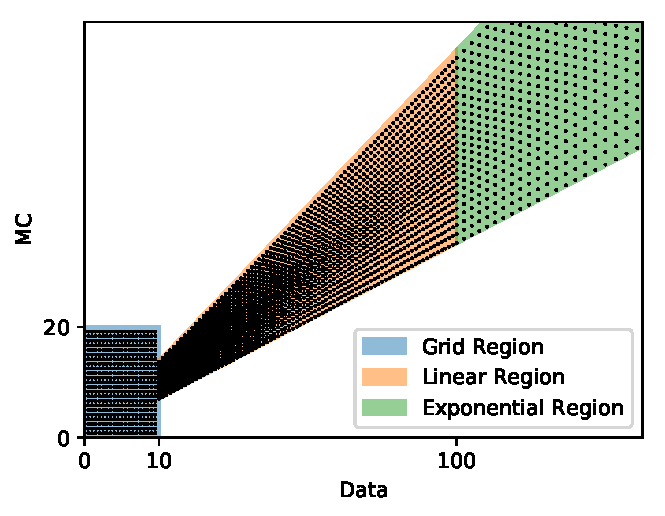
\includegraphics[width=0.7\textwidth]{lut/lut_points}
    \caption{Illustration of the point-density for various areas within the \ac{LUT}. Only the exact \TS values for the values indicated by the black dots are stored, interpolation is done in-between. The "grid region" is defined with equidistant spacing of exact \Ndata and \Nmc points. The "linear region" is equidistant in \Ndata, but two-sided exponential in \Nmc. In the "exponential region", the spacing between exact \Ndata points also grows exponentially.}
    \label{fig:lut_points}
\end{figure}

\subsubsection{Validation}
The \ac{LUT} can be easily validated by comparing \TS values from the complete calculation with \TS values obtained from the \ac{LUT} algorithm. Because the input domain for both algorithms is three-dimensional, we restrict ourselves to analyzing one-dimensional slices of the input domain and discuss its generality afterwards. The parameter values have been chosen to ensure the relative deviation $\frac{\abs{\TS_\text{LUT}-\TS}}{\TS}$ between the algorithms is less than \SI{1}{\percent}.

First, we vary the relative uncertainty while keeping \Ndata and \Nmc fixed. The results are shown in  \fref{fig:lut_reldiff_reluncert}. On the left hand side, \Ndata is fixed to \num{0}, while $\Nmc = \num{1}$. One can see that over the entire range of covered relative uncertainty (from \SI{0}{\percent} to \SI{130}{\percent}), the relative deviation between \ac{LUT} and full calculation is below \SI{0.1}{\percent}. 

Similarly, \fref{fig:lut_reldiff_mc} shows results from varying \Nmc over a fixed value of \Ndata and relative uncertainty. The dashed black line indicates the requirement of \SI{1}{\percent}. 

In both cases the relative differences show a repetitive pattern mostly below \SI{0.1}{\percent}. Except for a non-differentiable feature at $\Nmc = \Ndata$ and extreme values of \Nmc and low uncertainties, the maximum of the deviation lies below \SI{1}{\percent}, fulfilling the requirement. In the case of the extreme values, the low \TS value ($< \num{0.005}$) causes the \ac{LUT} value to be vetoed and the full calculation to take place. The repetitive pattern is also expected as it shows the high accuracy close to exactly calculated points and lower, but sufficient, accuracy in the linearly interpolated regions in between.

\begin{figure}
    \centering
    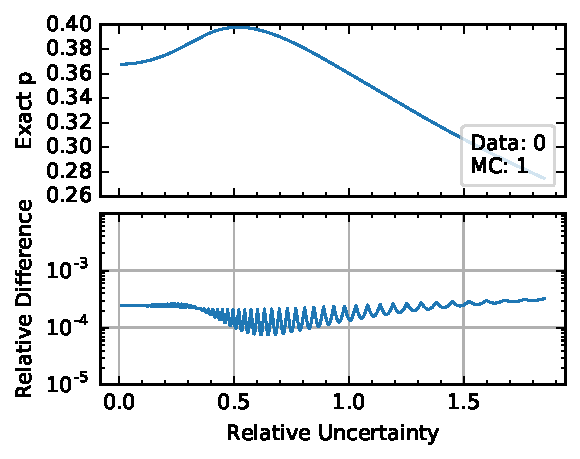
\includegraphics[width=0.49\textwidth]{lut/lut_uncert1}
    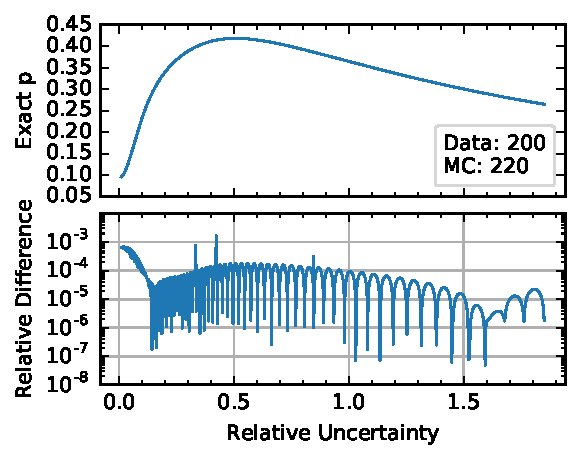
\includegraphics[width=0.49\textwidth]{lut/lut_uncert2}
    \caption{Relative difference between the complete calculation of \TS and results from the \ac{LUT}, varying the relative uncertainty while keeping \Ndata and \Nmc fixed. The relative difference is below \SI{0.1}{\percent} over the entire covered range.}
    \label{fig:lut_reldiff_reluncert}
\end{figure}


\subsubsection{Discussion}
Within the validated regions, the \ac{LUT} has only shown small deviations from the results of a full computation, orders of magnitude below the previously set threshold of \SI{1}{\percent}. Under these conditions it is therefore believed to provide a suitable alternative to the full computation of \TS values.

Performance measurements (see \fref{app:lut_performance}) indicate that the time spent on calculating \TS values, which was previously the dominating computational expense, has been reduced by a factor of $\approx \num{8}$. However, additional expenses arise, such as transferring the file to worker nodes and subsequently reading the file from the hard drive. The total gain will thus be less.

Overall, the \ac{LUT} contributes great value to the automated search, as a reduction in computing time allows us to increase the number of pseudo-experiments, enhancing the resolution of \ptilde values. In future developments of the analysis, we would suggest further optimization of the \ac{LUT} parameters, as they have only been roughly chosen to match the given requirements.

\begin{figure}
    \centering
    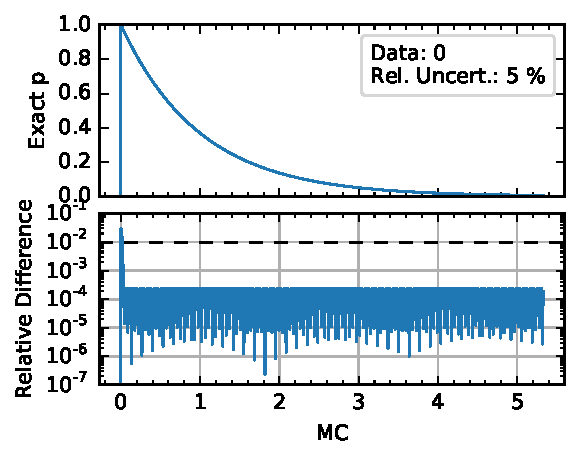
\includegraphics[width=0.4\textwidth]{lut/lut0a}
    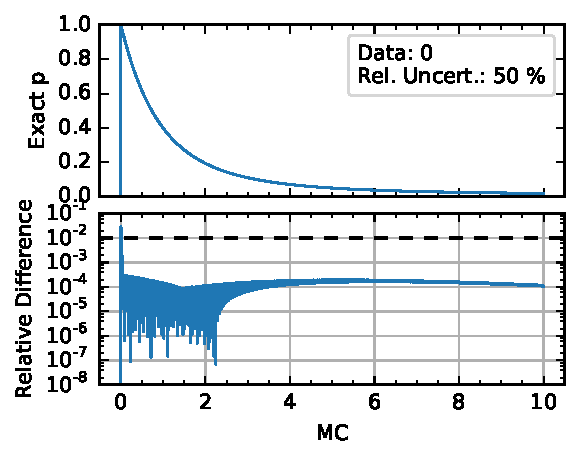
\includegraphics[width=0.4\textwidth]{lut/lut0b}
    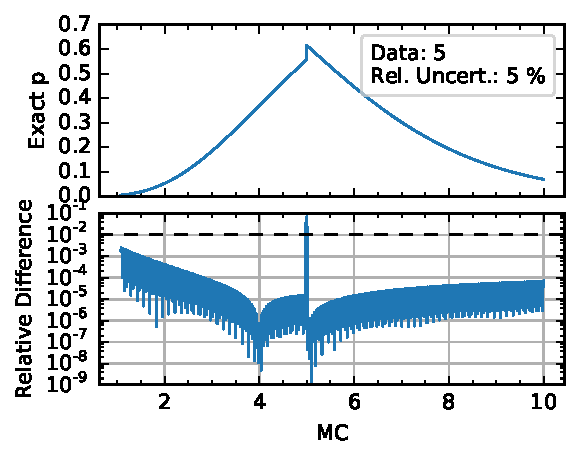
\includegraphics[width=0.4\textwidth]{lut/lut1a}
    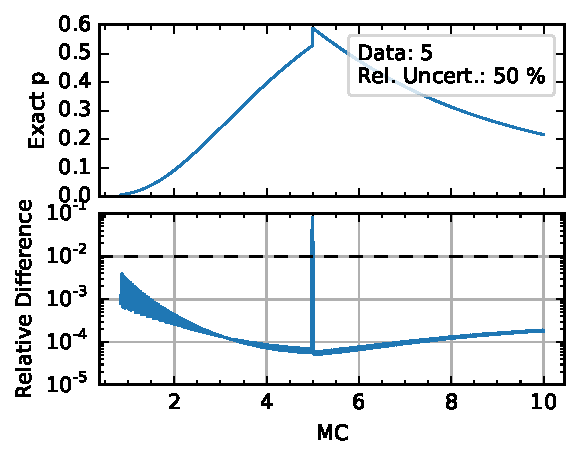
\includegraphics[width=0.4\textwidth]{lut/lut1b}
    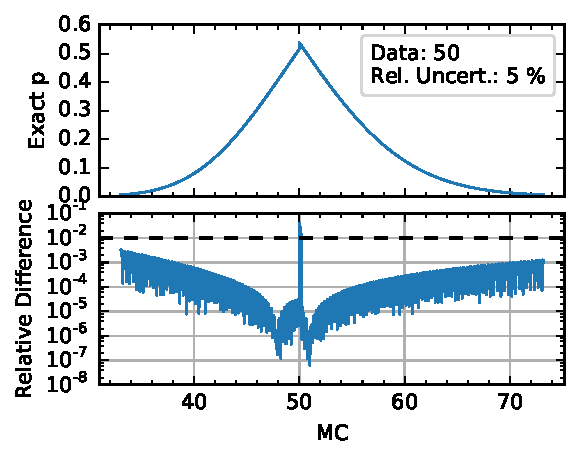
\includegraphics[width=0.4\textwidth]{lut/lut2a}
    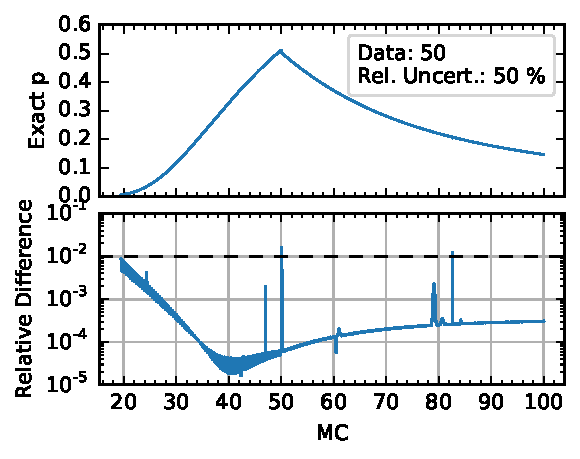
\includegraphics[width=0.4\textwidth]{lut/lut2b}
    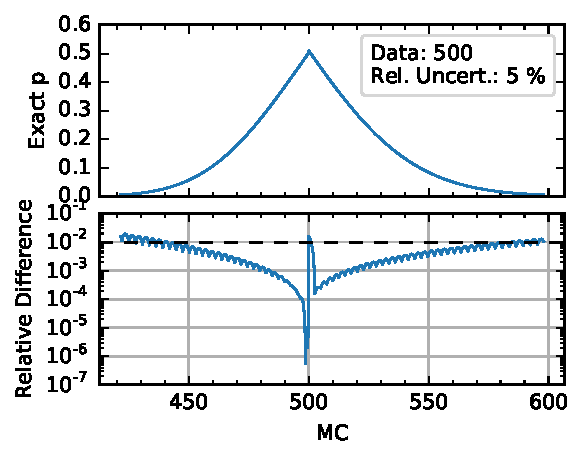
\includegraphics[width=0.4\textwidth]{lut/lut3a}  
    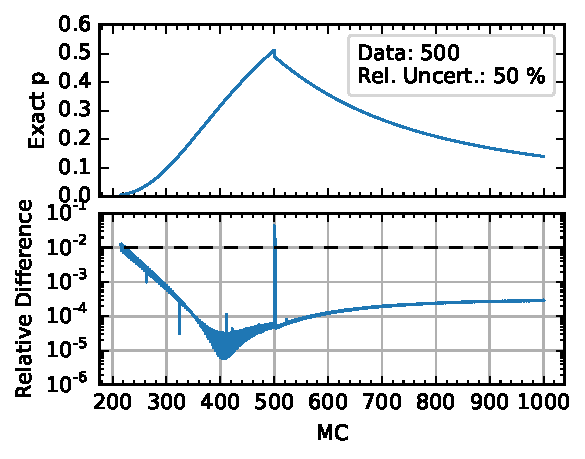
\includegraphics[width=0.4\textwidth]{lut/lut3b}
    \caption{Relative differences between the complete calculation of \TS and results from the \ac{LUT}, varying \Nmc while keeping \Ndata and the relative uncertainty fixed. The relative difference between the algorithms is below \SI{1}{\percent} (dashed line) in almost all regions.}
    \label{fig:lut_reldiff_mc}
\end{figure}